% vim:tw=72 sw=2 ft=tex
%         File: HW2.tex
% Date Created: 2016 Feb 11
%  Last Change: 2016 Feb 16
%     Compiler: make
%       Author: Adam Lang $ Gabriel Anderson Santiago
\documentclass[12pt,a4paper]{article}
\usepackage{amsmath, amssymb}
\usepackage[utf8]{inputenc}
\usepackage[T1]{fontenc}
\usepackage[english]{babel}
\usepackage{graphicx}

\graphicspath{{fig/}}

\title{Homework assignment 2 - EL2450}
\author{Adam Lang (861110-3956) \& Gabriel Andersson Santiago
(910706-4538)}

\begin{document}
\maketitle
\section{} %1
  Rate Monotonic scheduling is a scheduling method that will
  predetermine the priority of each task proportional to the tasks
  activation frequency. The priority is determined at the task creation
  and will remain unchanged during the whole application.

\section{} %2
  A set of tasks $J=\{J_1,J_2,...,J_n\}$ is schedulable with RM if
  \begin{equation}
    U=\sum\limits_{i=1}^n \frac{C_i}{T_i} \leq n(2^{1/n}-1)
  \end{equation}
  where $C_i$ is the comutation time, $T_i$ is the period, $U$ is the
  utilization factor and $n$ is the
  number of computations. When we have a sampling time of 
  $T=\{20, 29, 30\}ms$ and a computation time of 6 ms each we can see that,
  \begin{equation}
    \frac{6}{20}+\frac{6}{29}+\frac{6}{30}=0.707
  \end{equation}
  and with a utilization factor of $U = 0.780$ we can see that the set
  of tasks $J$ should be shedulable with RM.

\section{}%3
    \begin{center}
      \begin{figure}
        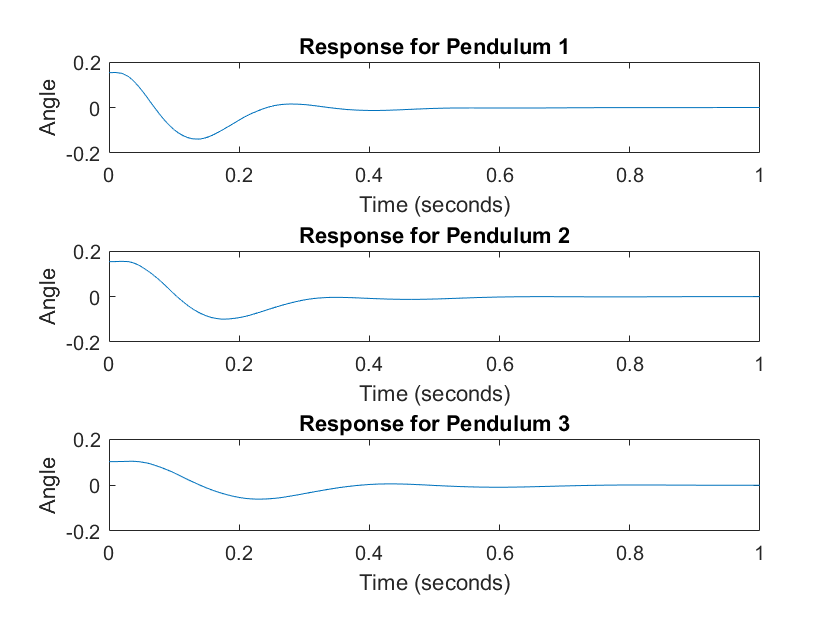
\includegraphics[scale=0.5]{ex31.png}
        \reference{fig:ex31}
      \end{figure}
        \caption{Pendulum angles for the three different pendulums}
    \end{center}
    
    \begin{center}
      \begin{figure}
        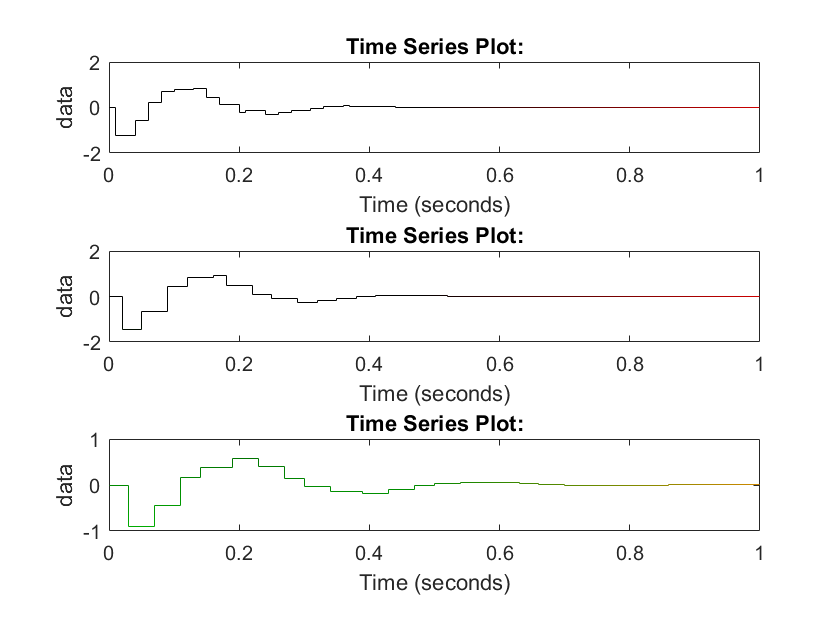
\includegraphics[scale=0.5]{ex32.png}
        \reference{fig:ex32}
      \end{figure}
      \caption{Control signal for pendulum}
    \end{center}

    The pendulums are indeed stabilized. There is however a slight difference
    in the control performance. From what we can see is the settling
    time longer the shorter the pendulum gets. Which is correct
    according to the lab introduction. 



\end{document}
